\begin{figure}[t]\centering
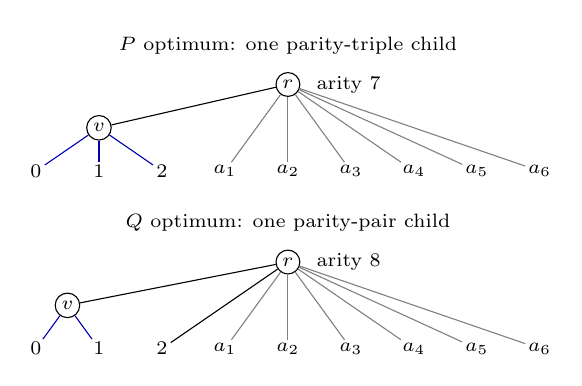
\begin{tikzpicture}[x=.8cm,y=.55cm,every node/.style={font=\scriptsize},
 root/.style={circle,draw,inner sep=1.3pt}, leaf/.style={inner sep=1pt}]
\node at (4,2.9) {$P$ optimum: one parity-triple child};
\node[root] (pr) at (4,2) {$r$};
\node[root] (pt) at (1,1) {$v$};
\node[right] at (4.3,2) {arity 7};
\foreach \x/\lab in {0/0,1/1,2/2,3/a_1,4/a_2,5/a_3,6/a_4,7/a_5,8/a_6}{
 \node[leaf] (p\x) at (\x,0) {$\lab$};}
\draw (pr)--(pt);
\foreach \x in {0,1,2}{\draw[blue!70!black] (pt)--(p\x);}
\foreach \x in {3,...,8}{\draw[gray] (pr)--(p\x);}
\node at (4,-1.2) {$Q$ optimum: one parity-pair child};
\node[root] (qr) at (4,-2.1) {$r$};
\node[root] (qt) at (.5,-3.1) {$v$};
\node[right] at (4.3,-2.1) {arity 8};
\foreach \x/\lab in {0/0,1/1,2/2,3/a_1,4/a_2,5/a_3,6/a_4,7/a_5,8/a_6}{
 \node[leaf] (q\x) at (\x,-4.1) {$\lab$};}
\draw (qr)--(qt);
\foreach \x in {0,1}{\draw[blue!70!black] (qt)--(q\x);}
\draw (qr)--(q2);
\foreach \x in {3,...,8}{\draw[gray] (qr)--(q\x);}
\end{tikzpicture}
\caption{Nine-leaf witness for Theorem~\ref{thm:pairwise-optimum}, with
$H=512,S=320,b=8$. The six anchors $a_i$ are distinct always-present
leaves, each a separate root child. Grouping the parity triple costs
3,856/4,224 refresh bytes under $P/Q$; grouping a pair costs 3,936
under either law. Construction adds 4,224 bytes to both trees.}
\label{fig:pairwise-witness}
\end{figure}
